\documentclass[pdftex,12pt, oneside]{article}

%\usepackage[paperwidth=8.5in, paperheight=13in]{geometry} % Folio
\usepackage[paperwidth=8.27in, paperheight=11.69in]{geometry} % A4

\usepackage{makeidx}         % allows index generation
\usepackage{graphicx}        % standard LaTeX graphics tool
                             % when including figure files
\usepackage[bottom]{footmisc}% places footnotes at page bottom
\usepackage[english]{babel}
\usepackage{enumerate}
\usepackage{paralist}
\usepackage{float}
\usepackage{gensymb}  
\usepackage{listings}
\usepackage{color}
\usepackage{mathtools} % atau \usepackage{amsmath}
\renewcommand{\baselinestretch}{1.5}

\newcommand{\HRule}{\rule{\linewidth}{0.5mm}}

\definecolor{codegreen}{rgb}{0,0.6,0}
\definecolor{codegray}{rgb}{0.5,0.5,0.5}
\definecolor{codepurple}{rgb}{0.58,0,0.82}
\definecolor{backcolor}{rgb}{0.95,0.95,0.92}

\lstdefinestyle{mystyle}{
  backgroundcolor=\color{backcolor},
  commentstyle=\color{codegreen},
  keywordstyle=\color{magenta},
  stringstyle=\color{codepurple},
  basicstyle=\footnotesize,
  breakatwhitespace=false,
  breaklines=true,
  captionpos=b,
  keepspaces=true,
  numbers=left,
  numbersep=5pt,
  showspaces=false,
  showstringspaces=false,
  showtabs=false,
  tabsize=2
}

\lstset{style=mystyle}


\begin{document}
\sloppy % biar section ga melebar melewati kertas

\begin{center}
{\large RANCANGAN RINCI SISTEM \textit{WEB SERVICES} SEBAGAI CARA KOMUNIKASI DENGAN TEMPAT PEMBAYARAN DALAM PENCATATAN PEMBAYARAN PAJAK BUMI DAN BANGUNAN PERDESAAN DAN PERKOTAAN DI KABUPATEN BREBES.}
\\[1cm]
DD MMM 2016\\
Priyanto Tamami, S.Kom.
\end{center}

%\frontmatter%%%%%%%%%%%%%%%%%%%%%%%%%%%%%%%%%%%%%%%%%%%%%%%%%%%%%%


%%%%%%%%%%%%%%%%%%%%%%%%%%%%%%%%%%%%%%%%%%%%%%%%%%%%%%%%%%%%%%%%%%%%%%

\section{SISTEM KOMPUTER}

Sistem komputer yang digunakan akan terbagi menjadi 3 (tiga) yaitu :

\begin{enumerate}[1.]
  \item Sebagai \textit{server} basis data adalah sebagai berikut :

    \begin{itemize}
      \item Prosesor Intel Xeon 2,4GHz
      \item Memori 44GB
      \item Sistem Operasi Windows Server 2008 R2 64 bit.
    \end{itemize}
    
  \item Sebagai \textit{server} aplikasi adalah sebagai berikut :
  
    \begin{itemize}
      \item Prosesor Intel Xeon 3,1GHz
      \item Memori 4GB
      \item Sistem Operasi CentOS 6.2 64 bit
    \end{itemize}
    
  \item Sebagai \textit{client} spesifikasi yang digunakan bebas, dapat menggunakan sistem komputer apapun yang dapat berkomunikasi melalui jaringan TCP/IP.
  
  Karena \textit{client} nantinya adalah Bank sebagai tempat pembayaran, maka sebagai sarana untuk uji coba dapat menggunakan sistem komputer apapun dengan \textit{browser} Chrome / Firefox.

\end{enumerate}

\section{SISTEM JARINGAN}

Sistem jaringan yang nantinya dibangun akan terlihat seperti pada gambar \ref{fig:network-diagram} :

\begin{figure}[H]
  \centering
  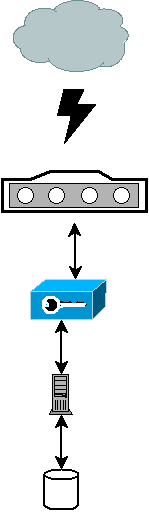
\includegraphics[width=0.5\textwidth]{./resources/diagram/network-diagram}
  \caption{Diagram Sistem Jaringan \textit{Web Services} PBB}
  \label{fig:network-diagram}
\end{figure}

Dari diagram tersebut, gambar awan adalah simbol untuk jaringan internet. Untuk melakukan akses ke \textit{server web service} akan melalui modem dibawahnya, kemudian akan menghubungi VPN \textit{server} terlebih dahulu untuk mendapatkan otentikasi atau akses ke dalam jaringan internal.

Setelah sukses melakukan otentikasi ke \textit{server} VPN, selanjutnya \textit{client} dalam hal ini Bank akan melakukan akses ke \textit{server web service} langsung, dimana \textit{server web service} akan melakukan komunikasi dengan \textit{server} basis data.

\section{SISTEM BASIS DATA}

Sistem basis data yang digunakan adalah sama dengan sistem basis data yang digunakan pada SISMIOP untuk pengelolaan PBB-P2, yaitu sistem basis data Oracle Database 11g. Namun tidak semua objek digunakan pada sistem \textit{web service} yang akan dibangun. Beberapa tabel yang digunakan adalah sebagai berikut :

\begin{itemize}
  \item Tabel SPPT
  
  Tabel SPPT ini nantinya hanya akan merubah pada kolom STATUS\_PEMBAYARAN\_SPPT, untuk isian 0 (nol) artinya nomor objek pajak (NOP) untuk tahun pajak tersebut belum dibayarkan, sedangkan isian 1 (satu) artinya NOP untuk tahun pajak tersebut sudah terbayar.
  
  \item Tabel PEMBAYARAN\_SPPT
  
  Tabel PEMBAYARAN\_SPPT ini apabila ada transaksi pembayaran, akan dicatatkan lengkap pada tabel ini, NOP apa, tahun pajak kapan, besarnya nilai yang dibayarkan, tanggal pembayaran, semuanya tersimpan pada tabel ini. Namun bila terjadi permintaan proses \textit{reversal}, maka data yang tersimpan pada tabel ini akan dihapuskan.
  
  \item Tabel LOG\_TRX\_PEMBAYARAN
  
  Tabel LOG\_TRX\_PEMBAYARAN ini digunakan untuk menyimpan aktivitas transaksi pembayaran yang sukses.
  
  \item Tabel LOG\_REVERSAL
  
  Tabel LOG\_REVERSAL digunakan untuk menyimpan aktivitas \textit{reversal} yang berhasil dilakukan pada basis data.
\end{itemize}

Beberapa \textit{store procedure} juga dibuat untuk mempercepat eksekusi proses, \textit{store procedure} ini, \textit{store procedure} yang dibuat adalah sebagai berikut :

\begin{itemize}
  \item SPPT\_TERHUTANG
  
  \textit{Store procedure} ini akan bertugas memberikan data SPPT terhutang ke aplikasi yang melakukan eksekusi terhadapnya.
  
  \item PROSES\_PEMBAYARAN
  
  \textit{Store procedure} ini akan bertugas melakukan pencatatan pembayaran pada tabel PEMBAYARAN\_SPPT, melakukan perubahan isi kolom STATUS\_PEMBAYARAN\_SPPT pada tabel SPPT, kemudian melakukan pencatatan prosesnya pada tabel LOG\_TRX\_PEMBAYARAN.
  
  \item REVERSAL\_PEMBAYARAN
  
  \textit{Store procedure} ini bertugas melakukan penghapusan data pada tabel PEMBAYARAN\_SPPT, merubah kolom STATUS\_PEMBAYARAN\_SPPT pada tabel SPPT menjadi 0 (nol), dan melakukan pencatatan pada tabel LOG\_REVERSAL.
\end{itemize}

\section{PROSEDUR AKTIVITAS}



% isinya :
%   - diagram use-case
%   - activity diagram
%   - class diagram
%   - entity relational diagram (db)
%   - sequence diagram
%   - deployment diagram

\section{SUMBER DAYA MANUSIA}

\end{document}